\documentclass[a4paper,10pt]{ltjsarticle}
\usepackage{graphicx}
\usepackage{luatexja-fontspec}
\usepackage{caption}
\usepackage{amsmath,amssymb,bm,braket,amsmath,latexsym, mathtools}
\usepackage[english]{babel}
\usepackage{physics}
\usepackage{multicol}
\usepackage{titlesec}
%\usepackage{gnuplot-lua-tikz}
\usepackage[top=20truemm,bottom=20truemm,left=20truemm,right=20truemm]{geometry}
\usepackage{array}
\usepackage{upgreek}
\usepackage{fancyhdr}
\renewcommand{\refname}{}
\usepackage{listings,jvlisting}
\usepackage{tikz}
\usepackage[version=3]{mhchem}
\usetikzlibrary{external}
\tikzexternalize
\lstset{
  basicstyle={\ttfamily},
  identifierstyle={\small},
  commentstyle={\smallitshape},
  keywordstyle={\small\bfseries},
  ndkeywordstyle={\small},
  stringstyle={\small\ttfamily},
  frame={tb},
  breaklines=true,
  columns=[l]{fullflexible},
  numbers=left,
  xrightmargin=0pt,
  xleftmargin=3pt,
  numberstyle={\scriptsize},
  stepnumber=1,
  numbersep=1pt,
  lineskip=-0.5ex
}
\captionsetup[figure]{format=plain, labelformat=simple, labelsep=quad,labelfont=bf,name={Fig.}}
\captionsetup[table]{format=plain, labelformat=simple, labelsep=quad,labelfont=bf}
\parindent = 0pt
%[BoldFont=HGSMinchoE]{MSMincho}[BoldFont=HiraMinProN-W6]{HiraMinPro-W3}
\pagenumbering{gobble}

\begin{document}
\centerline{\Large\bfseries unfolding Color Codeの誤り耐性 その2}
\vspace{10pt}
 前回に引き続き、Color Codeのunfolding操作について誤り耐性を調べてみた。特にunfoldingする際の折り目の部分のエラー検出に関して詳しく解析した。
\section{折り目付近の誤り耐性}{

    \begin{figure}[h]
        \centering
        \includegraphics[scale=0.2]{figure/figure1.eps}
        \caption{ }
        \label{figure1}
    \end{figure}

    前回までのunfolding操作をFig.\ref{figure1}に示す。前回の資料(unfolding\_color\_code\_2.pdf)ではあまり折り目の部分について議論しなかったが、よくよく考えてみると折り目の部分の誤り検出は思った以上に難しい。ここではそれを示す。\\
     まず、最初Color Codeから始まったとき、左上部分には$\ket{0}$初期化されているqubitが用意してある。つまり、それらのqubitは1-weight Z stabilizerでスタビライズされている。そのことを、水色をZ stabilizerとしてFig.\ref{figure2}(a)に示す。このとき、境界だけに注目すると、Fig.\ref{figure2}(b)に示すように、red face Z stabilizerと付近の1-weight Z stabilizerで六角形のZ stabilizerが構成できる。これより、unfolding操作の折り目をまたがる6-weight Z stabilizerによって折り目付近のXエラーを検出できる。

    \begin{figure}[h]
        \centering
        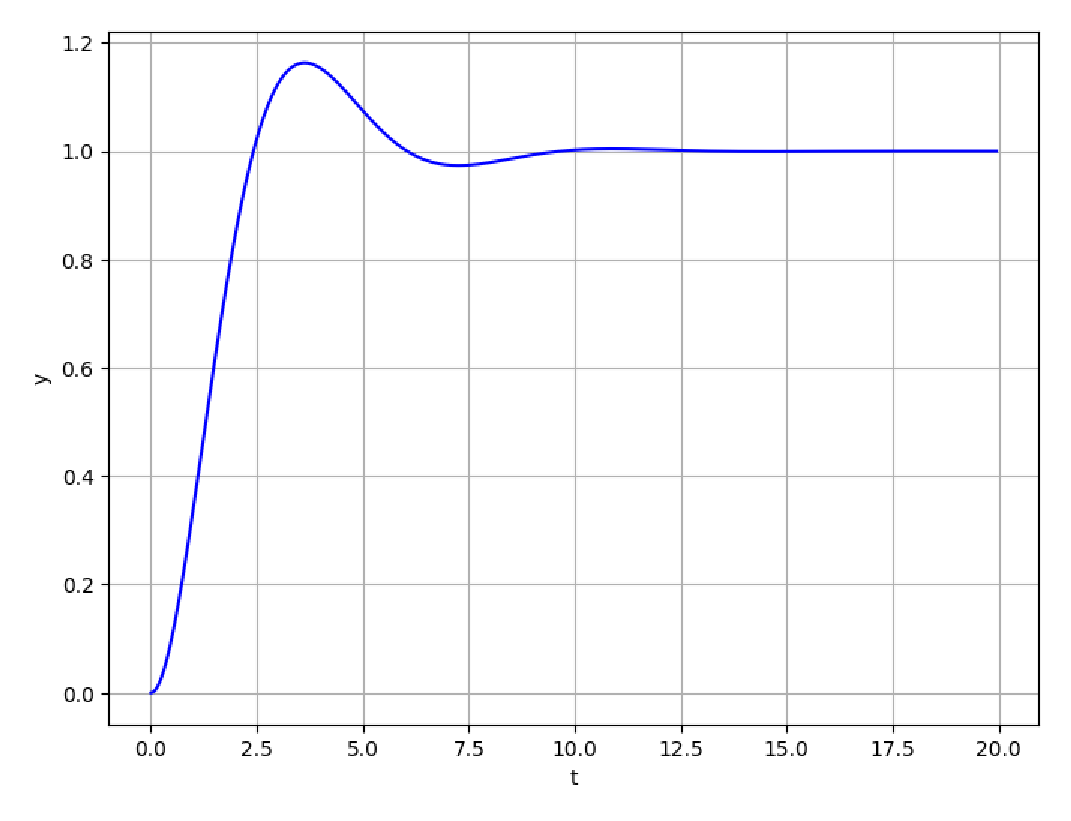
\includegraphics[scale=0.2]{figure/figure2.eps}
        \caption{ }
        \label{figure2}
    \end{figure}

    しかし、Fig.\ref{figure3}に示すような破線の6-weight Z stabilizerはundeterministicである。そのため、Fig.\ref{figure2}(b)の上の紫色の六角形のZ stabilizerで検出されたエラーはFig.\ref{figure3}のqubit 1,2,3,4のどこで起きたのかが全くわからない。そのようなことから、前回提示したunfoldingのプロトコルは折り目付近のXエラーが取り除けない。

    \begin{figure}[h]
        \centering
        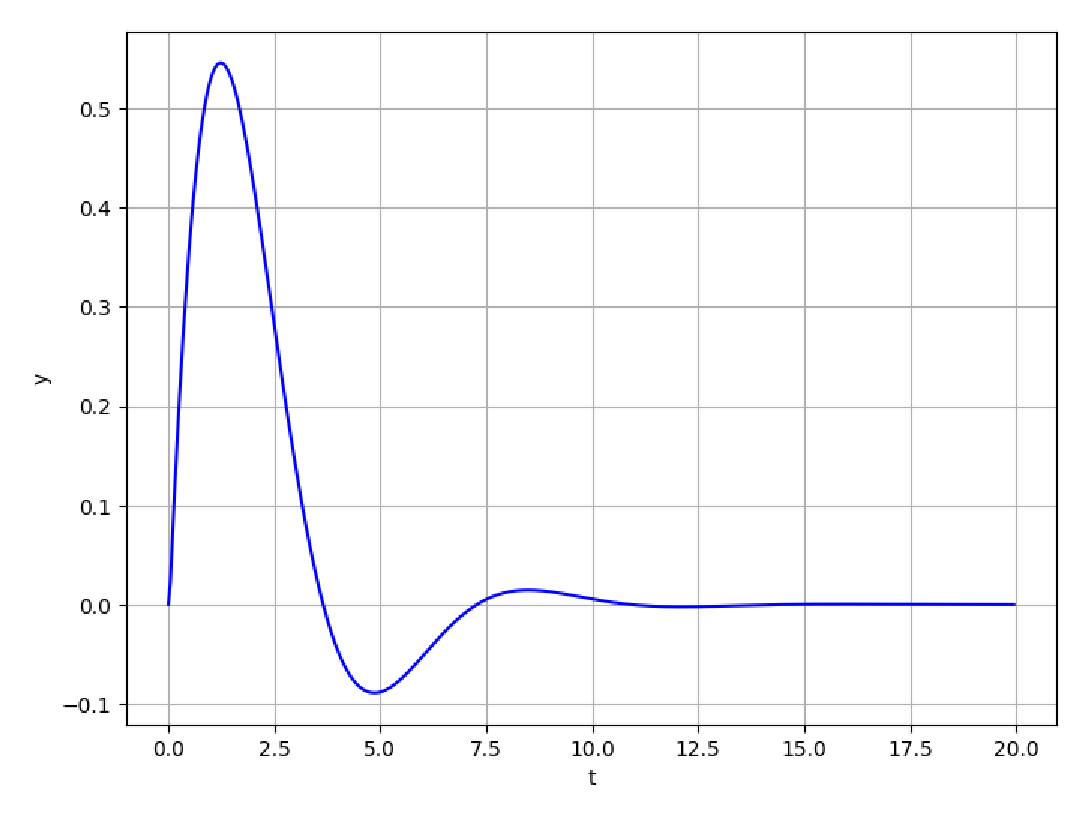
\includegraphics[scale=0.3]{figure/figure3.eps}
        \caption{ }
        \label{figure3}
    \end{figure}

    また、前回のプロトコルだと折り目付近のZエラーも取り除けないことに気がつく。しかしこれは、折り目付近の2つのqubitをBell 状態にすることによって解決する。それを紫色をX stabilizerとしてFig.\ref{figure4}に示す。ただし、このようにしても上記のXエラーを取り除けいない問題は残る。このとき、Bell状態のqubitのZエラーも取り除ける。
    
    \begin{figure}[h]
        \centering
        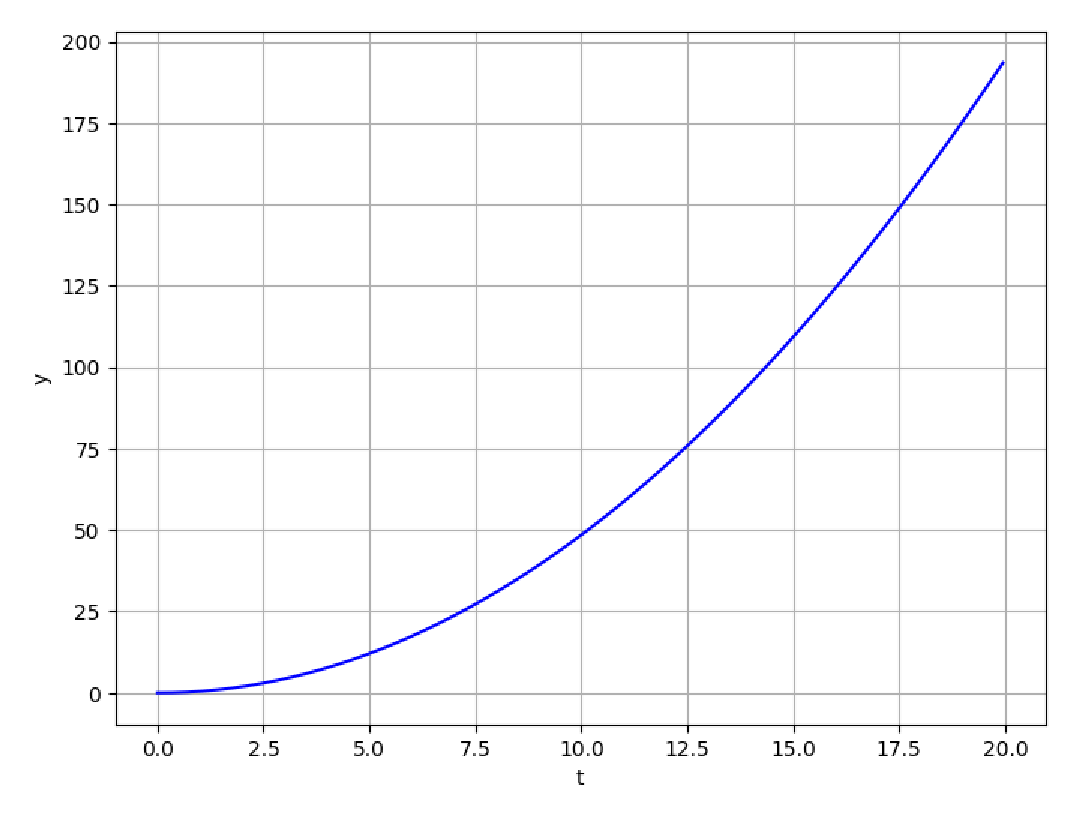
\includegraphics[scale=0.3]{figure/figure4.eps}
        \caption{ }
        \label{figure4}
    \end{figure}

    ということで現状のプロトコルは修正が必要である。参考までにFig.\ref{figure5}に試みた構造の残骸を載せておく。Fig.\ref{figure5}に示すどの構造をとっても(stabililzer自体が成り立っていないものもある)上記と似たような問題が発生した。

    \begin{figure}[h]
        \centering
        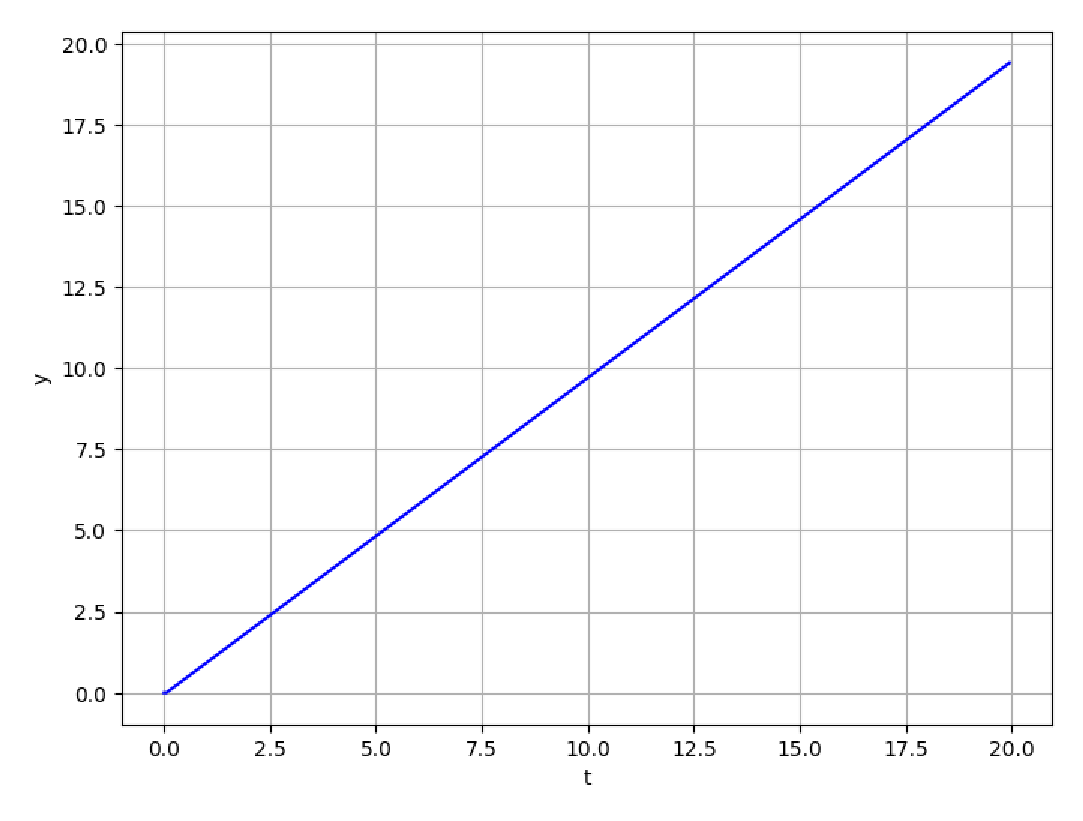
\includegraphics[scale=0.5]{figure/figure5.eps}
        \caption{ }
        \label{figure5}
    \end{figure}
}
\clearpage
 ということで上記の問題の解決策になりそうなものを思いついたのでそれを以下で述べる。
\section{Floquet Code}{
     解決策としてFloquet Codeを用いるやり方を思いついたので、まずトーラス上でのFloquet Codeを使ったColor Codeのunfoldingを考える。測定の種類や順番はFig.\ref{figure6}示す通りである。ここで、Fig.\ref{figure6}にはシンドローム測定するスタビライザーしか示していない。実際にはFig.\ref{figure6}はもっと多く示していないスタビライザーが存在する。

    \begin{figure}[h]
        \centering
        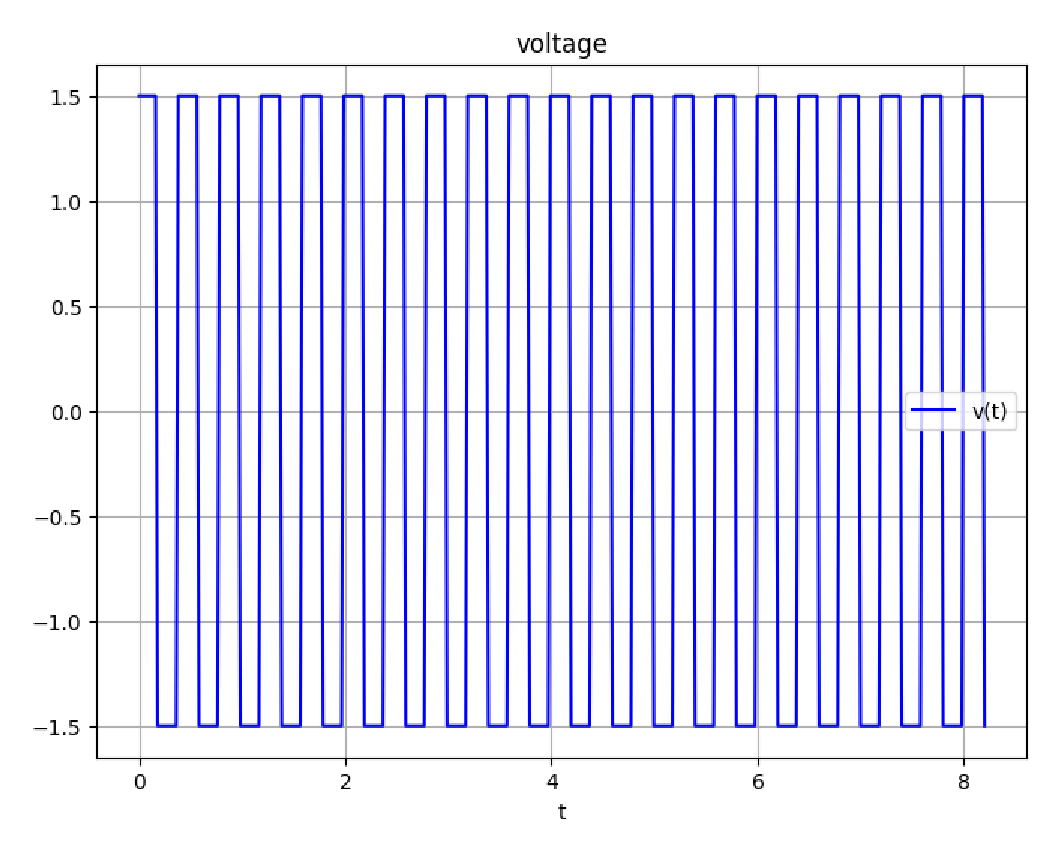
\includegraphics[scale=0.3]{figure/figure6.eps}
        \caption{ }
        \label{figure6}
    \end{figure}

    ここから先、(1),(2),(3),(4)はFig.\ref{figure6}の(1),(2),(3),(4)を表す。

}
\end{document}